%%%%%%%%%%%%%%%%%%%%%%%%%%%%%%%%%%%%%%%%%%%%%%%%%%%%%%%%%%%%%%%%%%%%%%%%%%%%%%%
% Chapter 3: Procedimiento experimental 
%%%%%%%%%%%%%%%%%%%%%%%%%%%%%%%%%%%%%%%%%%%%%%%%%%%%%%%%%%%%%%%%%%%%%%%%%%%%%%%

Para realizar los pertinentes experimentos hemos creado un programa en lenguaje Python, que para cada una de las cotas de error recibidas, halla el t\'ermino en el cual el resto del polinomio de Taylor pasa a ser menor que el error. Una vez hallado el grado del resto utiliza este valor para representar el polinomio de Taylor que es de un grado menos que el grado del resto.
Tambi\'en hemos creado un programa para que nos represente en una gr\'afica los polinomios de Taylor anteriormente hallados junto con el cos(x). Y otra gr\'afica que muestra el tiempo empleado en calcular cada polinomio y mostrarlo.

%++++++++++++++++++++++++++++++++++++++++++++++++++++++++++++++++++++++++++++++
\section{Descripci\'on de los experimentos}
\label{3:sec:1}

Para realizar distintos experimentos debemos cambiar las cotas de error con lo que lograremos que se generen distintos polinomios de Taylor. Y gracias a la representaci\'on gr\'afica podemos ver cuanto se aproximan estos polinomios a la funci\'on cos(x).
Otros experimentos posibles ser\'ian cambiar el valor del centro y tambi\'en cambiar el valor del punto donde debe ser evaluado. En ambos casos con un objetivo similar al primer experimento.
\\ \\ \\ \\ \\ \\ \\ \\ \\ \\ \\ \\ \\ \\

%++++++++++++++++++++++++++++++++++++++++++++++++++++++++++++++++++++++++++++++
\section{Resultados obtenidos}
\label{3:sec:2}
Todos los experimentos fueron realizados para cinco cotas de error, estas son: [0.4789, 0.0456, 0.00005, 0.000000005, 0.000000000007].\\ 

En primer lugar ejecutamos el programa con el centro fijado en el punto 0 y con un valor de 2 para el punto.
\begin{figure}[htb]
\begin{center}
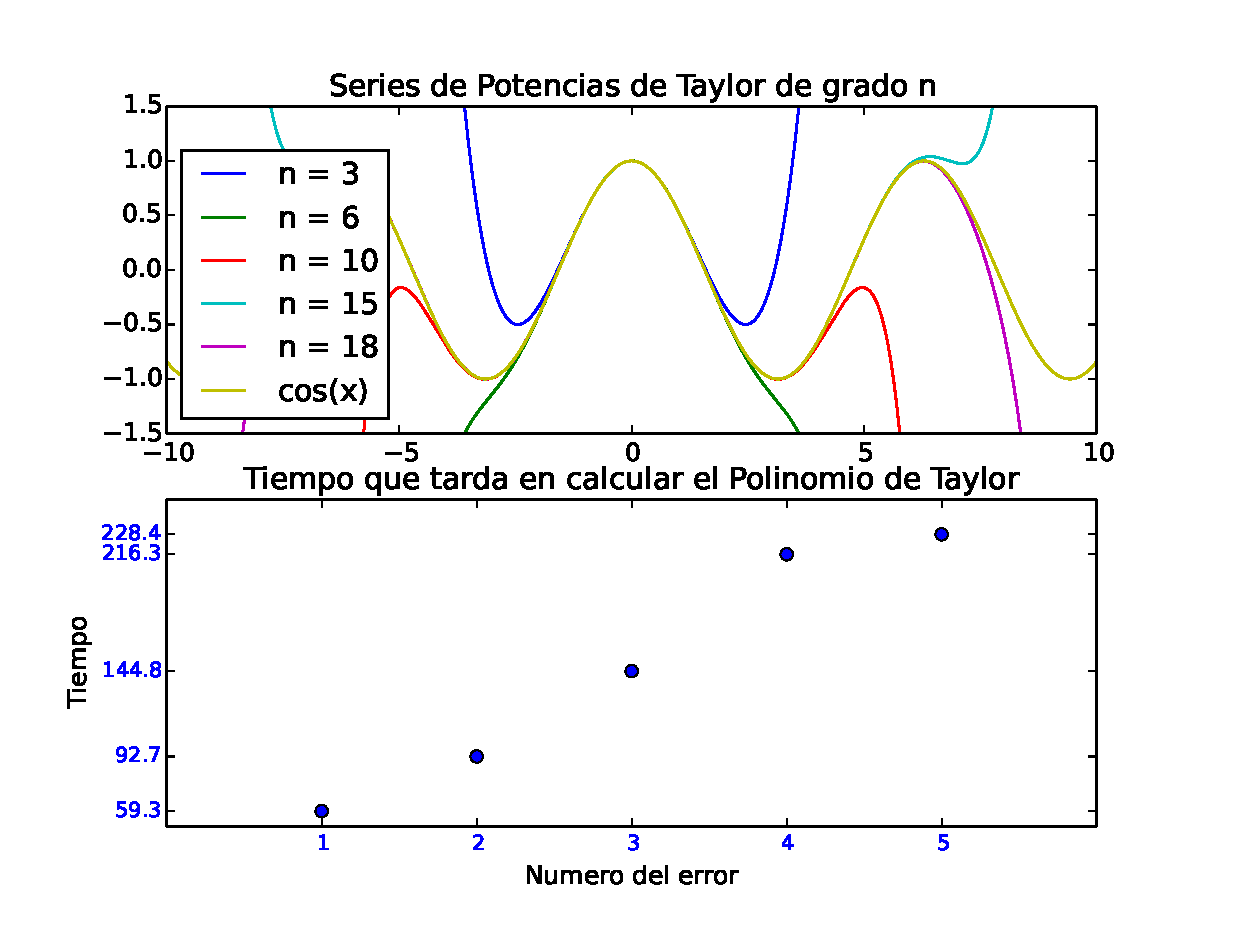
\includegraphics[width=10cm]{Graficas.eps}
\caption{Grafico de Taylor}
\label{fig}
\end{center}
\end{figure}

Podemos ver como cuanto mayor es el grado del polinomio la aproximaci\'on al coseno es mejor.\\ 

En segundo lugar hemos ejecutado el programa con el centro fijado en el punto 5 y con un valor de 2 para el punto.
\begin{figure}[htb]
\begin{center}
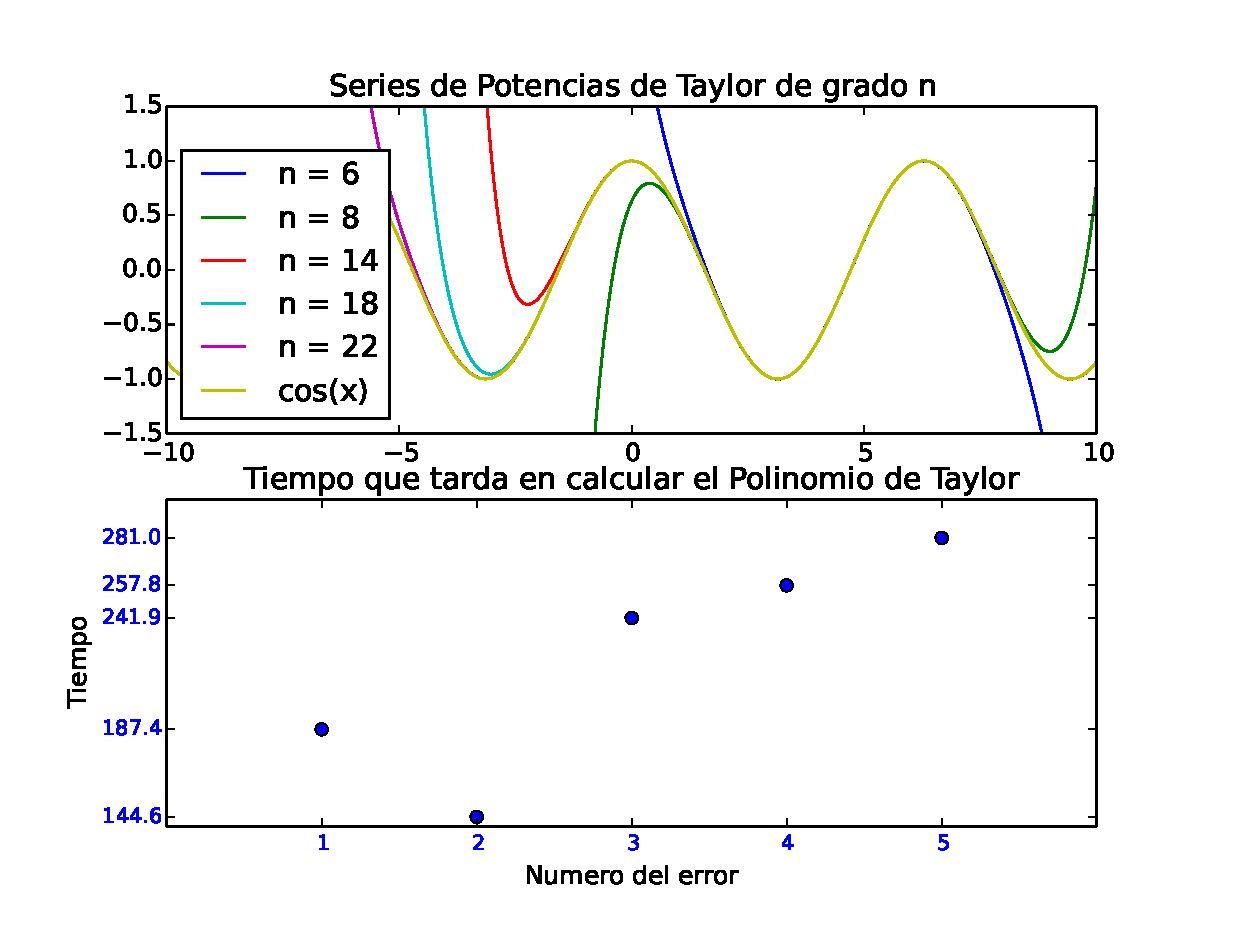
\includegraphics[width=10cm]{images/Graficascentro5.eps}
\caption{Valor del centro 5}
\label{fig}
\end{center}
\end{figure}
\\ \\ \\ \\ \\ \\ \\ \\ \\ \\ \\ \\ \\
En esta gr\'afica podemos ver como el polinomio aproxima al cos(x) pero siendo el punto 5 donde m\'as se aproxima dado que es el centro.\\
Por \'ultimo ejecutamos el programa con el centro fijado en el punto 0 y con un valor de 10 para el punto.
\begin{figure}[htb]
\begin{center}
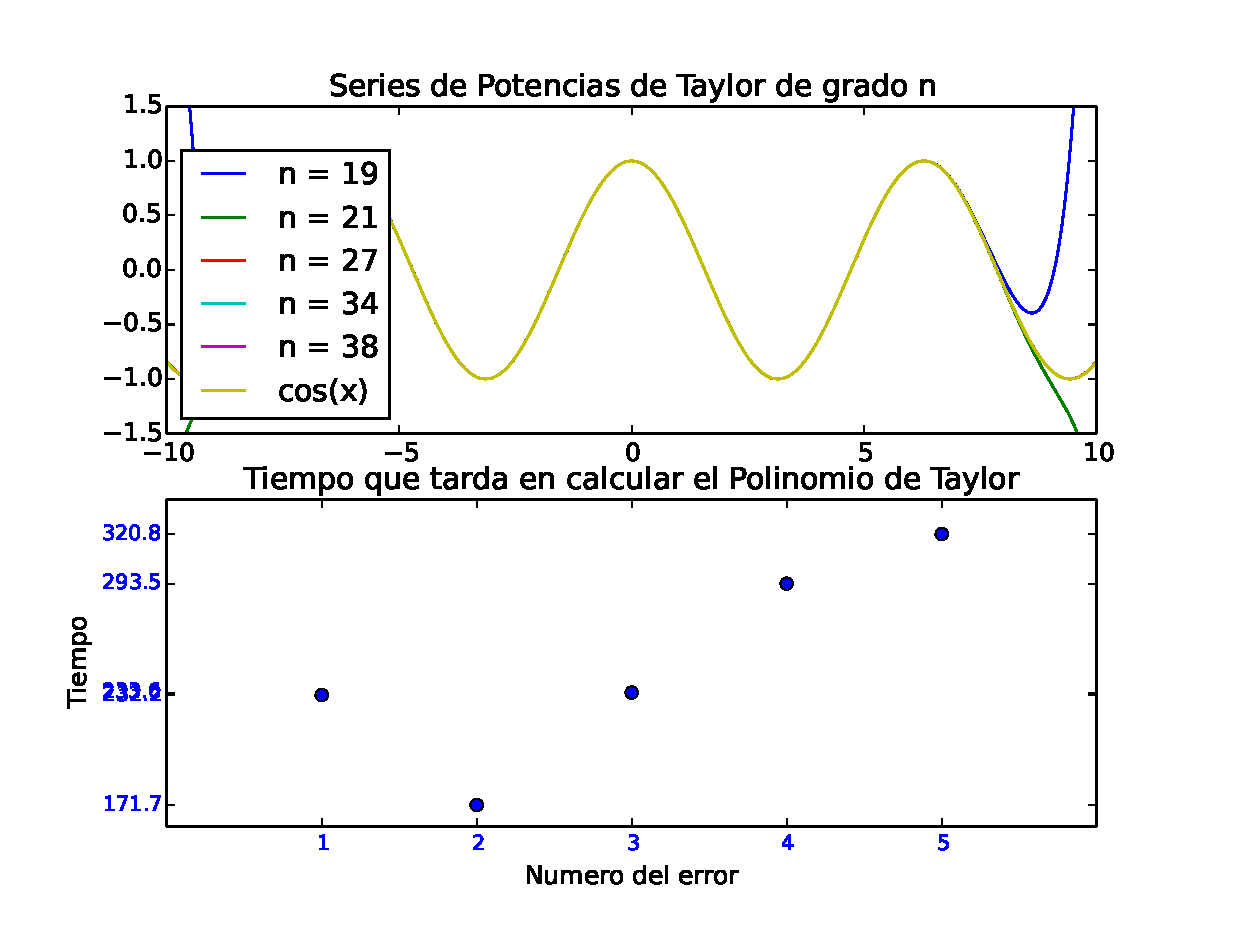
\includegraphics[width=10cm]{images/Graficas10.eps}
\caption{Valor del punto 10}
\label{fig}
\end{center}
\end{figure}